%%% License: Creative Commons Attribution Share Alike 4.0 (see https://creativecommons.org/licenses/by-sa/4.0/)
%%% Slides are based heavily on earlier versions of this course taught by Jesper Rudiger.

\documentclass[english,10pt]{beamer}
%\documentclass[english,10pt,handout]{beamer}
%%% License: Creative Commons Attribution Share Alike 4.0 (see https://creativecommons.org/licenses/by-sa/4.0/)
%%% Slides are based heavily on earlier versions of this course taught by Jesper Rudiger and Peter Norman Sorensen.

\DeclareGraphicsExtensions{.eps, .pdf,.png,.jpg,.mps,}
\usetheme{reMedian}
\usepackage{parskip}
\makeatother

\renewcommand{\baselinestretch}{1.1} 

\usepackage{amsmath, amssymb, amsfonts, amsthm}
\usepackage{enumerate}
\usepackage{hyperref}
\usepackage{url}
\usepackage{bbm}
\usepackage{color}

\usepackage{tikz}
\usepackage{tikzscale}
\newcommand*\circled[1]{\tikz[baseline=(char.base)]{
		\node[shape=circle,draw, inner sep=-20pt] (char) {#1};}}
\usetikzlibrary{automata,positioning}
\usetikzlibrary{decorations.pathreplacing}
\usepackage{pgfplots}
\usepgfplotslibrary{fillbetween}
\usepackage{graphicx}

\usepackage{setspace}
%\thinmuskip=1mu
%\medmuskip=1mu 
%\thickmuskip=1mu 


\usecolortheme{default}
\usepackage{verbatim}
\usepackage[normalem]{ulem}

\usepackage{apptools}
\AtAppendix{
	\setbeamertemplate{frame numbering}[none]
}
\usepackage{natbib}




\title{Financial Markets Microstructure \\ Lecture 4}

\subtitle{Liquidity and Price Dynamics\\
Chapter 3.4-3.7 of FPR}

\author{Egor Starkov}

\date{K{\o}benhavns Unversitet \\
	Spring 2020}


\begin{document}
	
\AtBeginSection[]{
\frame<beamer>{
\frametitle{This lecture:}
\tableofcontents[currentsection,currentsubsection]
}}

\frame[plain]{\titlepage}


\section{Revision and problems}

\begin{frame}{What did we do last week?}
\begin{enumerate}
	\item Information and prices
	\item Efficiency and markets
	\item Glosten and Milgrom: Workhorse model to analyze adverse selection in markets
	\begin{itemize}
	\item Analysis of what drives the spread
	\item Tradeoff between market liquidity and price discovery
	\item The model had reasonably good efficiency properties
	\end{itemize}
\end{enumerate}
\end{frame}


\begin{frame}[label=exercises]
\frametitle{Exercises from last time}
\begin{itemize}
	\item FPR chapter 3 exercises (p. 124-125):
	\begin{itemize}
		\item exercise 2 -- solve GM model with numbers instead of letters
		\item exercise 3 about the GM model where speculators are not perfectly informed, but instead receive a signal about the value of the asset
	\end{itemize}
	\item Will do this Friday.
\end{itemize}
\end{frame}


\begin{frame}{Today}
\begin{enumerate}
	\item Look at other drivers of the spread
	\begin{itemize}
		\item Order-processing costs
		\item Dealer inventory risk
	\end{itemize}
	\item We'll look at how their dynamic effect on prices differ
\end{enumerate}
\end{frame}



\section{Order-processing costs}

\begin{frame}{What order-processing costs exist?}
	A liquidity supplier (for instance a dealer) can have a range of different order-processing costs
	\begin{itemize}
		\item Trading fees:  charged by exchanges
		\item Clearing and settlement fees:  paid if a central clearinghouse is used to minimize trading risks
		\item Overheads: back office expenses
		\item (Dealer rents)
	\end{itemize}
	These costs must somehow be compensated by traders, and will therefore enter the spread
\end{frame}


\begin{frame}{How do these costs affect the spread?}
	\begin{itemize}
		\item Let $\mu_t \equiv \mathbb{E}[v | \Omega_t]$ be the expectation of $v$ \textit{after} the time-$t$ trade order is observed, and let $s^a_t$ and $s^b_t$ denote the `half-spreads'
		\item Hence, $\mu_{t-1}$ represents what we now when period $t$ starts
		\item  Then in the GM model  we can write prices as
		\begin{align*}
		a_{t} = \mu_{t-1} +s^{a}_{t} \\
		b_{t} = \mu_{t-1} - s^{b}_{t}
		\end{align*}
		\item Assume dealer has order cost $\gamma$, and charges this directly to trader:
		\begin{align*}
		a_{t} = \mu_{t-1} + \gamma + s^{a}_{t} \\
		b_{t} = \mu_{t-1} - \gamma - s^{b}_{t}
		\end{align*}
	\end{itemize}
\end{frame}


\begin{frame}{How do these costs affect the spread? (2)}
	\begin{itemize}
		\item  Hence, the new bid-ask spread is 
		\[
		S_{t} = a_{t} - b_{t} = 2\gamma +s^{a}_{t}  + s^{b}_{t}
		\]
		\item The spread is now made up of order costs ($2\gamma$) and adverse selection costs ($s^{a}_{t}  + s^{b}_{t}$)
		\item Suppose we want to determine whether spread in a given market is due to adverse selection or order costs
		\begin{itemize}
			\item The instantaneous effect of order costs is similar to that of adverse selection costs
			\item But we shall see that the dynamic effect is different
		\end{itemize}
	\end{itemize}
\end{frame}


\begin{frame}{The dynamics of the spread}
	\begin{itemize}
		\item As before, let $d_{t}=1$ denote a buyer-initiated trade, and $d_{t} = -1$ a seller-initiated trade
		\item Also, let $s(d_{t})$ be the adverse-selection-related half-spread depending on the trade: $s(1)=s^{a}_{t}$ and $s(-1)=s^{b}_{t}$
		\item Then the realized price can be written as
		\[
		p_{t} = \mu_{t-1} + (s(d_{t}) + \gamma) d_{t}
		\]
		\item Since $\mu_{t} = \mu_{t-1} + s(d_{t}) d_{t}$, then
		\[
		p_{t}  = \underbrace{\mu_{t}}_{\structure{\text{updated valuation}}} + \underbrace{\gamma d_{t}}_{\structure{\text{order cost}}}
		\]
	\end{itemize}
\end{frame}


\begin{frame}{The dynamics of the spread}
	Then the effect of time-$t$ trade on prices:
	\begin{itemize}
		\item \textbf{short-run}: $$p_t - \mu_{t-1} = (s(d_{t}) + \gamma) d_{t}$$
		\item \textbf{long-run}:
		\begin{align*}
			\mathbb{E}_t [p_{t+s}] - \mu_{t-1} &= \mathbb{E}_t [\mu_{t+s-1} + (s(d_{t+s}) + \gamma) d_{t+s}] - \mu_{t-1}
			\\
			&\approx \mathbb{E}_t [\mu_{t+s-1}] - \mu_{t-1}
			\\
			&= \mu_t - \mu_{t-1}
			\\
			&= s(d_t) d_t
		\end{align*}
		\item so order cost effect on prices is \emph{transient} and is reversed by future trades;
		\item effect of adverse selection term is \emph{permanent}
	\end{itemize}
\end{frame}


%\begin{frame}{The dynamics of the spread (2)}
%	\begin{itemize}
%		\item The resulting deviation from the midprice $|p_{t}-\mu_{t}|=\gamma$ is \textit{transient}: it is unrelated to fundamentals
%		\item In the GM model, the price is a martingale: the expectation of tomorrow's price is today's price
%		\item What about here? 
%		\item \textbf{Short-run impact}: Suppose a 'buy' order at time $t$. Compare realized price to ideal 'liquid' price $\mu_{t-1}$:
%		\[
%		p_{t}  - \mu_{t-1} = a_{t} - \mu_{t-1} = s^{a}_{t} + \gamma
%		\]
%		This is the short-run impact on prices
%	\end{itemize}
%\end{frame}
%
%
%\begin{frame}{Dynamics: textbook version}
%	\begin{itemize}
%		\item \textbf{Long-run impact}. Say we look at the effect $T$ periods ahead:
%		\begin{align*}
%		\mathbb{E}[p_{t+T}|\Omega_{t-1}, d_{t}=1]
%		& = \mathbb{E}[\mu_{t+T}+ \gamma d_{t+T}|\Omega_{t-1}, d_{t}=1] \\
%		& = \mu_{t} + \gamma \mathbb{E}[d_{t+T}|\Omega_{t-1}, d_{t}=1] \\
%		& = \mu_{t-1} + s^{a}_{t}+ \gamma \mathbb{E}[d_{t+T}|\Omega_{t-1}, d_{t}=1] 
%		\end{align*}
%		\item Suppose $T$ is large. Then today's trade doesn't say much about trades at $T$:
%		\[
%		\mathbb{E}[d_{t+T}|\Omega_{t-1}, d_{t}=1]  \simeq 0
%		\]
%		{\small (Note: this is ``common sense'' statement, not from GM model -- there, conditional on $v$, $\mathbb{E}[d_t]$ is the same for all $t$ and is not zero in general.)}
%		\item So long-run effect is close to zero:
%		\[
%		\mathbb{E}[p_{t+T}|\Omega_{t-1}, d_{t}=1] - \mu_{t-1} \simeq s^{a}_{t}
%		\]
%	\end{itemize}
%\end{frame}
%
%
%\begin{frame}{Dynamics: textbook version (2)}
%	\begin{block}{}
%		\[
%		SR \, Impact - LR \, Impact = \gamma
%		\]
%	\end{block}
%	\begin{itemize}
%		\item Thus, the buy at time $t$ will increase prices, but afterwards there will be a \textit{price reversal}
%		\item If we are smart investors and know this, we will know that the price is above its long-run level
%		\item Can we make money off that? \pause \structure{No. In long run we expect price to fall by $\gamma$ after a buy, and rise by $\gamma$ after sale. No profit opportunity}
%	\end{itemize}
%\end{frame}
%
%
%\begin{frame}{Dynamics: alternative version}
%	\begin{itemize}
%		\item Think about how a buy affects next period's ask price. 
%		\item To do this, suppose $a^*_{t+1}$ is the ask price after a buy, and $a^0_{t+1}$ is the ask price if there is no trading at $t$. Recall that 
%		\begin{align*}
%		a_{t+1} & = \mu_t + s^a_{t+1} + \gamma \\
%		\mu_t & = \mu_{t-1} + s(d_t) d_t
%		\end{align*}
%		\item Thus:
%		\[
%		a^*_{t+1} - a^0_{t+1} = s^a_{t}
%		\]
%		Adverse selection is incorporated into future prices, order-processing costs are not
%	\end{itemize}
%% draw a graph on the board?
%\end{frame}



\section{Inventory risk}

\begin{frame}{Introduction: Stoll (1978)}
	\begin{itemize}
		\item Model of illiquidity due to dealers' asset inventory cost
		\item Competitive market makers/dealers (price takers)
		\begin{itemize}
			\item Risk averse, have an optimal portfolio of risky assets
			\item Submit their competitive demand schedule (limit orders)
		\end{itemize}
		\item Noise traders place market orders (no speculation)
		\begin{itemize}
			\item Orders contain no information about $v$
			\item Dealers are the counterparty, must be willing to change their portfolio
		\end{itemize}
		\item We model risk aversion. This may be due to the dealer's preferences, or due to regulation
	\end{itemize}
\end{frame}


\begin{frame}{Model}
	\begin{itemize}
		\item \textbf{Asset}. Single risky asset
		\begin{itemize}
			\item Current fundamental value $\mu_t$
			\item Held for one period by dealers, final value $v=\mu_t + \epsilon_t$
			\item Here $\mathbb{E}[\epsilon_t] = 0$ and $\mathbb{V}(\epsilon_{t})=\sigma^2_\epsilon > 0$
		\end{itemize}
		\item \textbf{Dealer}. Representative dealer
		\begin{itemize}
			\item Endowed with $z_t$ units of the risky asset
			\item Has cash holding $c_t$
		\end{itemize}
		\item \textbf{Competitive asset demand/supply}. Dealer acts as price taker.
		\begin{itemize}
			\item Given asset price $p_t$, supply $y_t$ units of asset
			\item Has utility defined over (random) next period wealth
			\[
			w_{t+1} = v(z_t - y_t) + c_t + p_t y_t
			\]
		\end{itemize}
	\end{itemize}
\end{frame}


\begin{frame}{Case 1: Mean-variance preferences}
	\begin{itemize}
		\item Suppose the dealer has mean-variance preferences:
		\[
		U(w_{t+1})=\mathbb{E}[w_{t+1}] - \frac{\rho}{2} \mathbb{V}(w_{t+1}),
		\]
		where $\rho>0$ measures risk aversion
		\item Dealer chooses $y_t$ to maximize
		\[
		\underbrace{\mu_t(z_t-y_t) + c_t + p_t y_t}_{\mathbb{E}[w_{t+1}] } - \frac{\rho}{2} \underbrace{(z_t -y_t)^2 \sigma^2_\epsilon}_{ \mathbb{V}(w_{t+1})}
		\]
		\item Solved by \structure{asset supply function}
			\[
			y_t = z_t + \frac{p_t-\mu_t}{\rho \sigma^2_\epsilon}
			\]
	\end{itemize}
\end{frame}


\begin{frame}{Case 1: Mean-variance preferences (2)}
	\begin{itemize}
		\item Define the midquote $m_t$ as the price where $y_t=0$,
		\[
		0 = z_t + \frac{m_t-\mu_t}{\rho \sigma^2_\epsilon}.
		\]
		Then the supply schedule (limit order book) is 
		\[
		y_t = \frac{p_t - m_t}{\rho \sigma^2_\epsilon}
		\]
		\item Equivalently, $p_t-m_t=\rho \sigma^2_\epsilon y_t$. We can think of this as a price impact equation where $\lambda=\rho \sigma^2_\epsilon$ (recall that $\lambda$ measures inverse depth)
		\item Greater depth $1/\lambda$ when dealers are more risk-tolerant ($\rho$ lower)
	\end{itemize}
\end{frame}


\begin{frame}{Case 2: Mean-SD preferences}
	\begin{itemize}
		\item Suppose the dealer dislikes standard deviation:
		\[
		U(w_{t+1})=\mathbb{E}[w_{t+1}] - \rho \sqrt{\mathbb{V}(w_{t+1})}.
		\]
		\item Dealer chooses $y_t$ to maximize
		\[
		\mu_t (z_t - y_t) + c_t + p_t y_t - \rho |z_t - y_t|\sigma_\epsilon
		\]
		\item This utility is linear in $y_t$. In particular,
		\[
		\frac{\partial U(w_{t+1})}{\partial y_t}= \left\{
		\begin{aligned}
		p_t-\mu_t+\rho\sigma_{\epsilon}	& \text{ if } z_t>y_t \\
		p_t-\mu_t-\rho\sigma_{\epsilon}	& \text{ if } z_t<y_t 
		\end{aligned}
		\right.
		\]
	\end{itemize}
\end{frame}


\begin{frame}{Case 2: Mean-SD preferences (2)}
	\begin{itemize}
		\item Given $\frac{\partial U(w_{t+1})}{\partial y_t}$, the dealer's optimal supply is
		\begin{itemize}
			\item Supply any $y_t \leq z_t$ if $p_t = \mu_t - \rho\sigma_{\epsilon}$,
			\item Supply any $y_t \geq z_t$ if $p_t = \mu_t + \rho\sigma_{\epsilon}$
		\end{itemize}
		\item There is a discountinuos `jump' in the price at $y_t=z_t$
		\begin{itemize}
			\item But otherwise supply perfectly elastic
		\end{itemize}
		\item A natural measure of the bid-ask spread is $2\rho\sigma_{\epsilon}$ if $z_t \simeq 0$
	\end{itemize}
\end{frame}


\begin{frame}{Conclusion: Stoll}
	\begin{itemize}
		\item In the Glosten-Milgrom model, the transactions price is always the expected asset value given trade history
		\item In the Stoll model, the price is moved by incoming random noise trades, and the midprice deviates from expected value in proportion to the inventory $z$, e.g.
		\[
		m_t - \mu_t = \rho \sigma^2_\epsilon z_t
		\]
		To emphasize: prices in Stoll model are \structure{not efficient}
		\item The difference can be interpreted as a risk premium to the  dealers
		\item Can you benefit from this as a trader? \pause \structure{Yes, in the sense that you can buy cheaper if you happen to look for a trade that reduces dealer risk exposure}
	\end{itemize}
\end{frame}


\begin{frame}{Liquidity risk in practice: \\Saxo Bank and the Swiss Franc}
	\begin{itemize}
		\item Saxo Bank had a  large and profitable brokering business, offering customers (leveraged) trading in Swiss Francs
		\item When the Franc abandoned its peg to the euro on 15 Jan 2015, many of these customers were facing huge losses and sought to get out of their positions fast
		\item The forex market is an \textit{over-the-counter} market: brokers quote prices and then try to fill those orders
	\end{itemize}
\end{frame}


\begin{frame}{Saxo Bank and the Swiss Franc}
	\begin{center}
		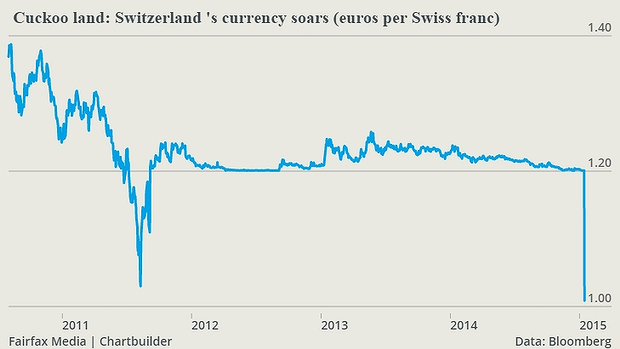
\includegraphics[width=0.6\linewidth]{pics/Francageddon_Image}
	\end{center}
	\begin{itemize}
		\item Liquidity dropped: Saxo found it hard to fill orders at quoted prices
		\item Saxo revised prices on trades \textit{after} the market had closed (legal?)
		\item Conclusion: Brokers face a substantial risk in illiquid markets - their quotes might go `stale'
	\end{itemize}
\end{frame}


\begin{frame}{Price dynamics with illiquidity}
	\begin{itemize}
		\item In practice, incoming market orders may, in the short run, move the transaction price beyond the update in expected value
		\begin{itemize}
			\item This is not due to adverse selection
			\item The effect may die out rapidly if caused by trading commissions/fees
			\item The effect may die out more slowly if caused by risk-averse dealers who slowly bring back their positions toward a target holding $z^*$
		\end{itemize}
		\item More on the speed of price discovery in chapter 5
	\end{itemize}
\end{frame}


\begin{frame}{Price dynamics}
	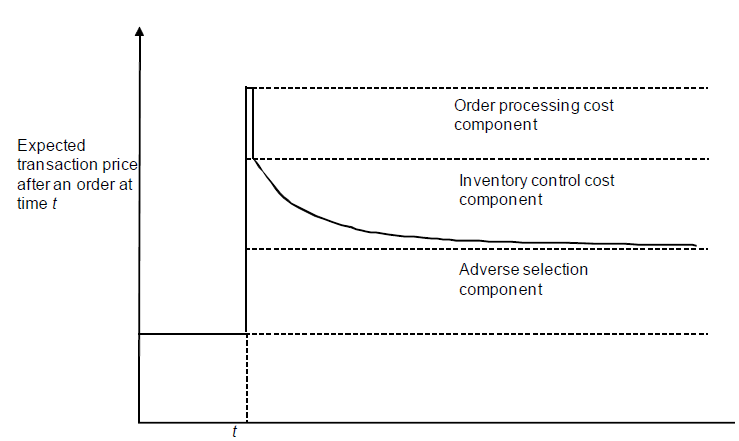
\includegraphics[width=0.9\linewidth]{pics/PriceDiscovery_Image}
\end{frame}


\begin{frame}{Summary}
	\begin{itemize}
		\item The spread is not only driven by adverse selection: order costs and inventory risk have an effect as well
		\item However, we would expect the dynamic effect of these three different mechanisms to be different
		\begin{itemize}
			\item Order costs: only instantaneous effect 
			\item Inventory risk: medium-run effect, but should be zero in the long run
			\item Adverse selection/information: long-run effect 
		\end{itemize}
		\item Next week we exploit this to estimate the importance of each mechanism
	\end{itemize}
\end{frame}


\begin{frame}{Exercises}
	\begin{itemize}
		\item for next Wednesday:
		\begin{itemize}
			\item In Absalon, I have attached an article from the Economist, December 14 2013, on the Volcker rule. Discuss the claim that \emph{``In practice banks will probably respond by making markets for a narrow range of securities that already trade frequently, and thus might reasonably be expected to do so in the future. Meanwhile, the securities that now change hands less frequently are likely to be shunned, making them even harder to trade.''}
			\item Two other Bloomberg articles are on Einar Aas and his exclusion from Nasdaq. Use this case to discuss how risk aversion can stem from regulation.
		\end{itemize}
		\item for this Friday:
		\begin{itemize}
			\item If you are bored, solve Exercise 9 on page 128 about the bid-ask spread in the mean-SD model
			\item If you feel like a challenge, solve exercise 10 on page 128
		\end{itemize}
	\end{itemize}
\end{frame}


\end{document} 